\section{Dynamic Exponent-Window Accumulation}
\label{sec:design}

\subsection{Partial-Sum Concentration and DEWA}
We observed the distribution of partial sums in LLaMA2-7B.
Three representative layers under the BFP4 format were selected for illustration.
The partial-sum distribution remains highly concentrated, indicating that a low-cost accumulator with a narrow dynamic range can be introduced prior to forwarding data to the FP-Acc.

Specifically, we define an accumulation window
\begin{equation}
    [E_{\max} - T_d,\; E_{\max} + T_r]
    \label{eq:window}
\end{equation}
where $E_{\max}$ denotes the exponent of the current maximum partial sum, and $T_d$ and $T_r$ represent the drop and replace thresholds, respectively.
When a new partial sum arrives:
\begin{itemize}
    \item if its exponent falls below the lower bound, it is discarded;
    \item if it exceeds the upper bound, it directly replaces the value currently held in the accumulator;
    \item otherwise, it is accumulated using the low-cost accumulator.
\end{itemize}
This approach substantially reduces FP-Acc utilization and thereby lowers power consumption~\cite{bucketgetter2023,winacc2025}.
We refer to this method as \textbf{Dynamic Exponent-Window Accumulation (DEWA)}.

\begin{figure}[t]
    \centering
    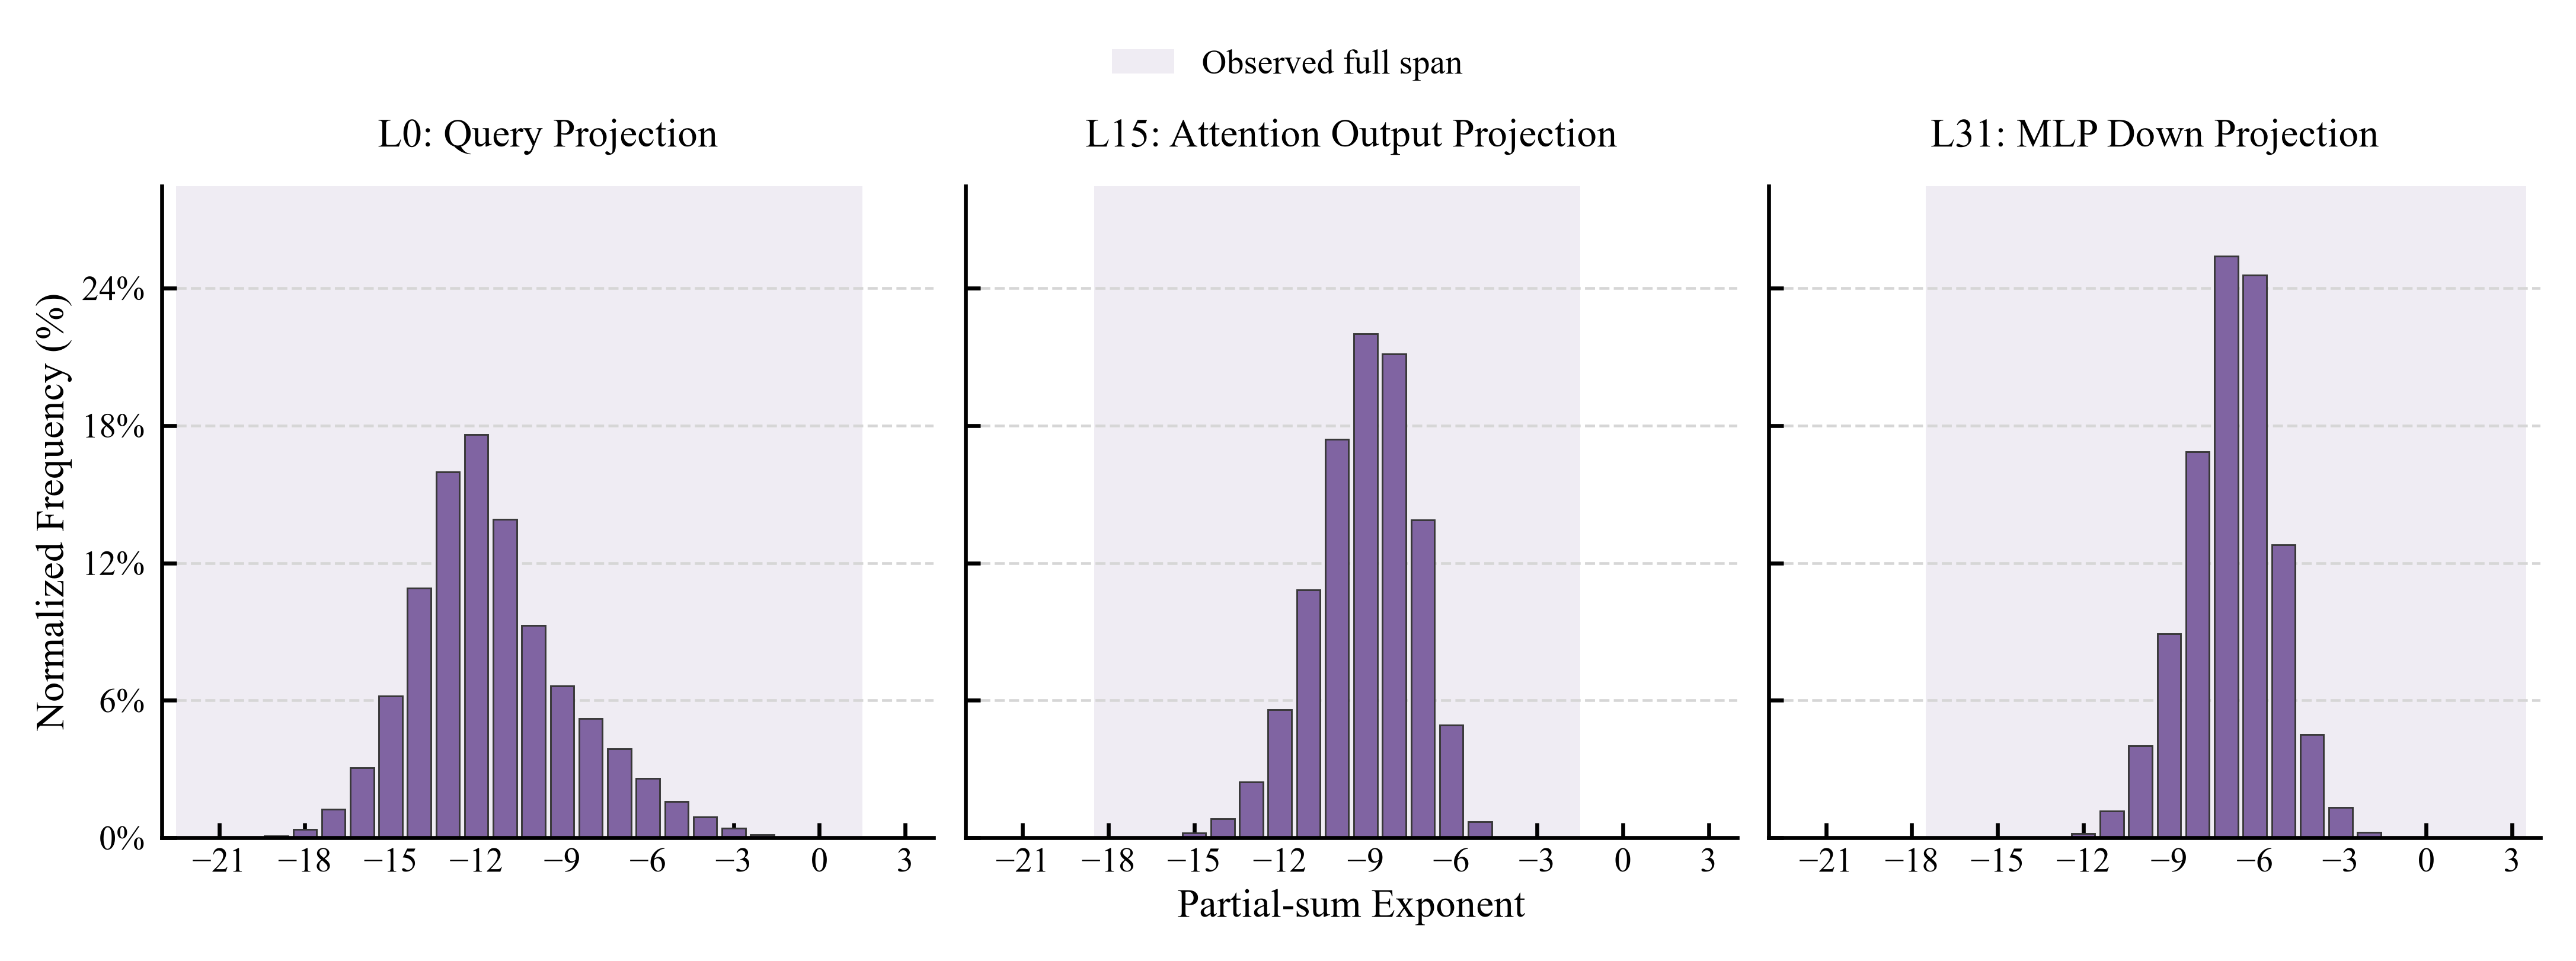
\includegraphics[width=\linewidth]{figures/fig_psum_distribution.png}
    \caption{Representative partial-sum exponent distributions under BFP4 (LLaMA2-7B, G16).}
    \label{fig:psum_profile}
\end{figure}

Although the majority of partial sums are concentrated, the overall distribution still exhibits a large dynamic range.
We attribute this to the influence of outliers, which cause the dynamic exponent window to shift significantly and thereby induce precision loss.
We therefore argue that outlier separation is essential as a complement to DEWA.
By separating activation outliers, a substantially higher proportion of partial sums fall within the accumulation window (Fig.~\ref{fig:in_window_rate}).

\begin{figure}[t]
    \centering
    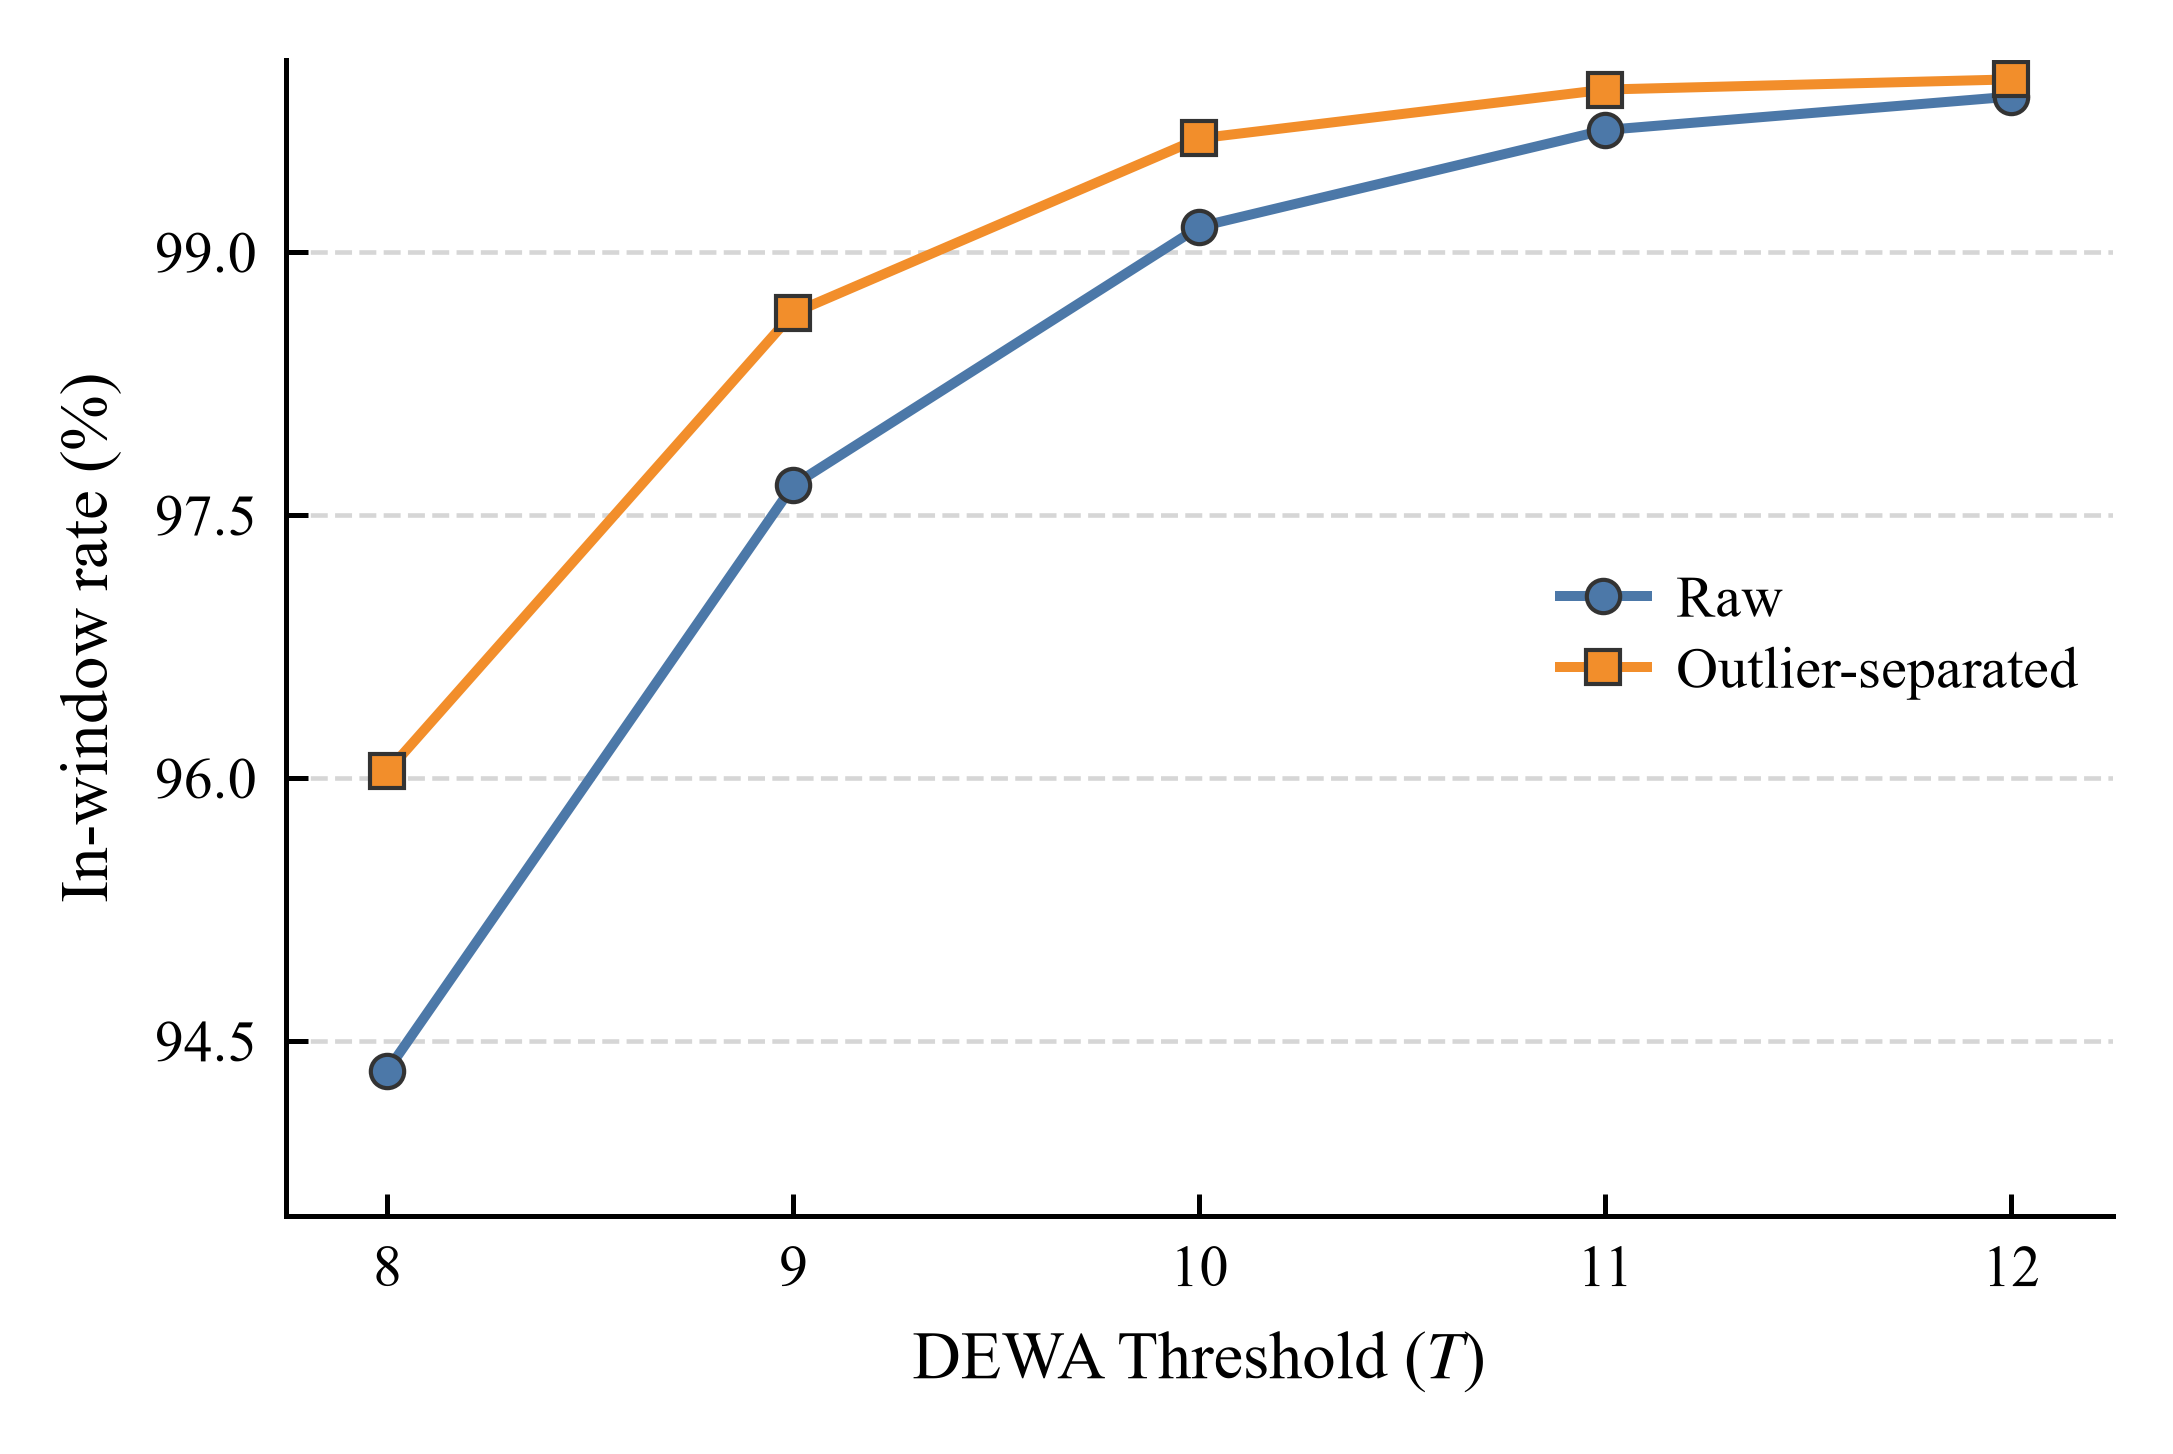
\includegraphics[width=\linewidth]{figures/fig_in_window_rate.png}
    \caption{DEWA in-window rate with and without outlier separation (BFP4, G16, $T=8$--$12$).}
    \label{fig:in_window_rate}
\end{figure}

\subsection{Activation Top-2 Selection}
In prior work, BiE~\cite{bie2024} and Oiso~\cite{oiso2026} employed a dual-exponent format to separate the exponents of normal values and outliers, prepending a type bit to each element to indicate its category.
While this format achieves notable accuracy improvement, it also introduces non-trivial overhead: since the proportion of outliers is inherently low, allocating an additional exponent and type bit to every element---combined with four distinct MAC cases---increases hardware cost.
Directly integrating this scheme into DEWA is therefore suboptimal.

Building on this observation, we introduce two improvements:
\begin{enumerate}
    \item Since the majority of outliers concentrate on specific activation channels, applying dual-exponent encoding to weights yields benefits that do not justify the associated overhead.
    We therefore adopt single-exponent BFP for weights while retaining dual-exponent encoding for activations.
    \item We further examined the number of outliers occurring within each block.
    Approximately 99.5\% of blocks contain at most two outliers.
    We propose \textbf{Activation Top-2 Selection}, wherein at most the two largest outliers are selected per block, further reducing hardware overhead.
\end{enumerate}

Fig.~\ref{fig:data_format} illustrates the resulting W-BFP4 / Top-2 A-BiE4 encoding.

\begin{figure}[t]
    \centering
    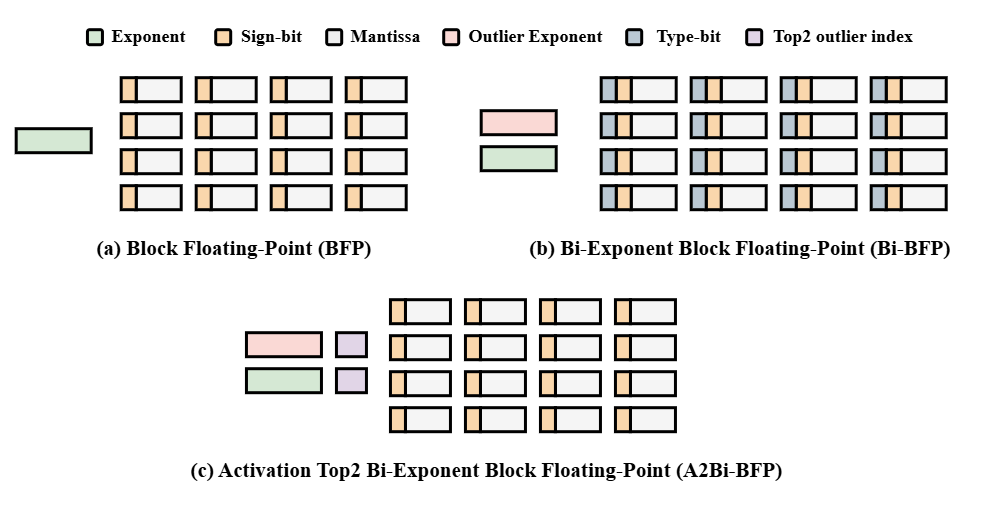
\includegraphics[width=\linewidth]{figures/fig_data_format.png}
    \caption{Data format for W-BFP4 weights and Top-2 A-BiE4 activations (G16).}
    \label{fig:data_format}
\end{figure}

\begin{table}[t]
    \centering
    \caption{Outlier occupancy per G16 activation block (W-BFP4/A-BiE4, LLaMA2-7B).}
    \label{tab:outlier_count}
    \begin{tabular}{lc}
        \toprule
        Statistic & Value \\
        \midrule
        Activation outlier rate & 0.913\% of lanes \\
        Affected blocks & 11.40\% of blocks \\
        Mean outliers per affected block & 1.28 \\
        Blocks with exactly one outlier & 86.10\% of affected \\
        All-block P99 outlier count & 2 \\
        \bottomrule
    \end{tabular}
\end{table}

Fig.~\ref{fig:ppl_improvements} summarizes the impact of activation-only BiE and Top-2 capping on LLaMA2-7B perplexity, where negligible degradation is observed relative to full BiE.

\begin{figure}[t]
    \centering
    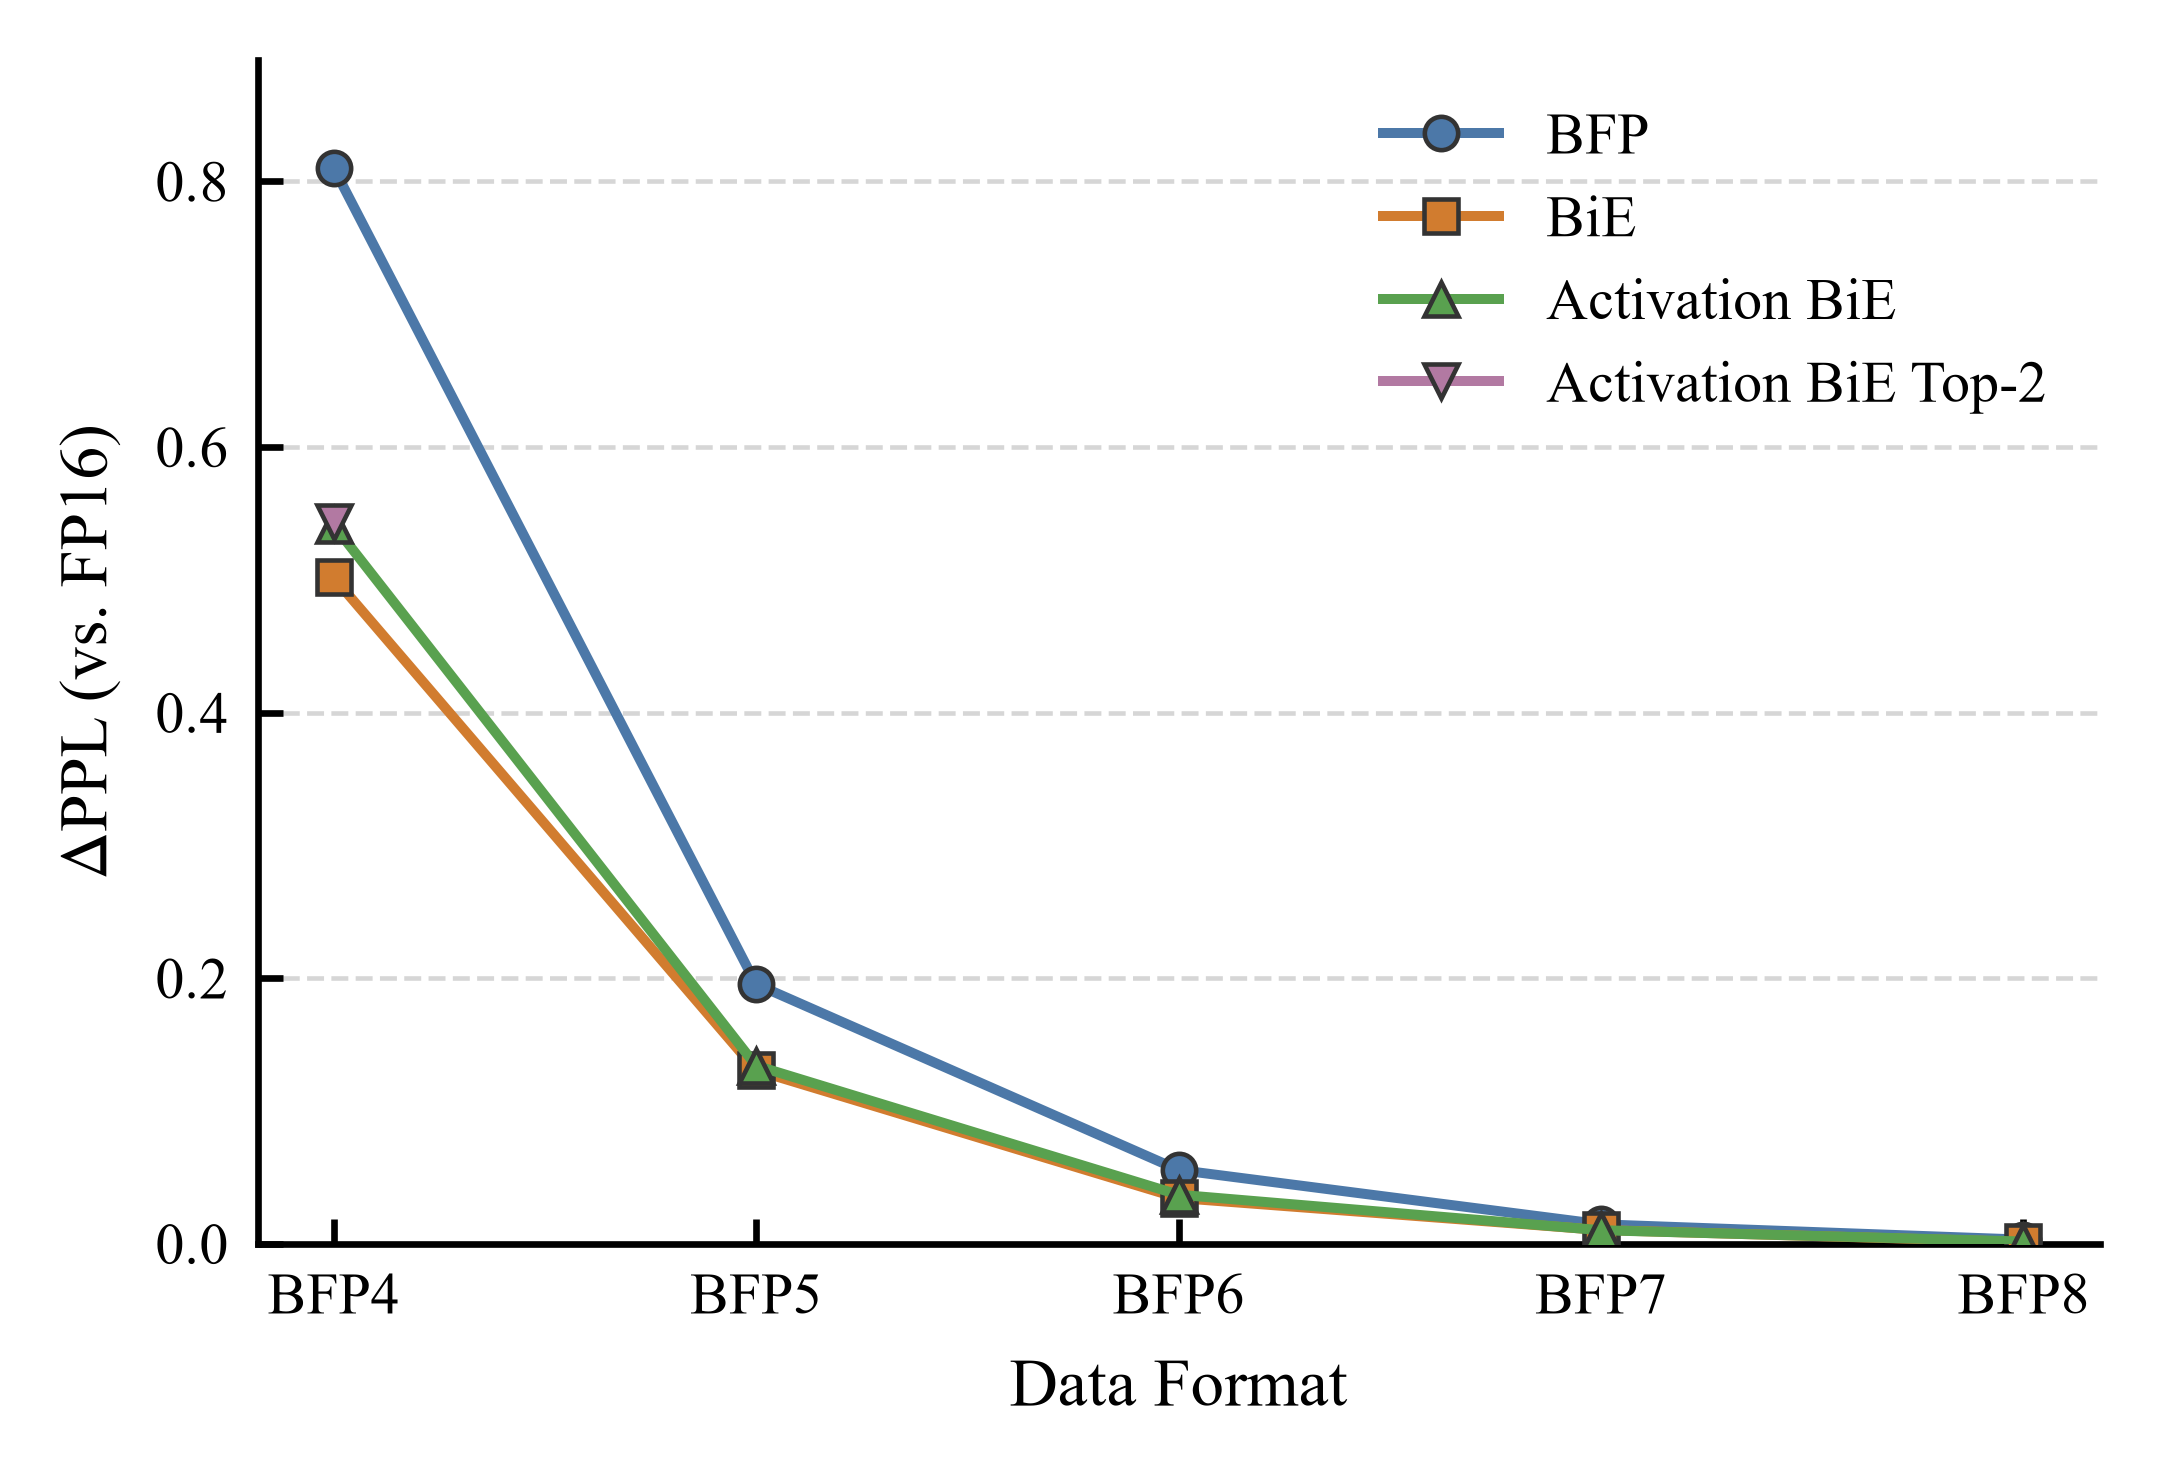
\includegraphics[width=\linewidth]{figures/fig_ppl_delta.png}
    \caption{Perplexity delta versus FP16 baseline for vanilla BFP, BiE, activation-only BiE, and Top-2 activation BiE.}
    \label{fig:ppl_improvements}
\end{figure}

\subsection{Hybrid Accumulation Flow}
The canonical hybrid design combines W-BFP4 weights, Top-2 A-BiE4 activations, G16 grouping, asymmetric DEWA thresholds ($T_{\mathrm{skip}}$, $T_{\mathrm{replace}}$), and direct exception routing to the FP-Acc.
For each output element within a G16 group, normal and outlier partial sums follow separate accumulation paths before a shared FP-Acc merges exception updates.

\begin{figure}[t]
    \centering
    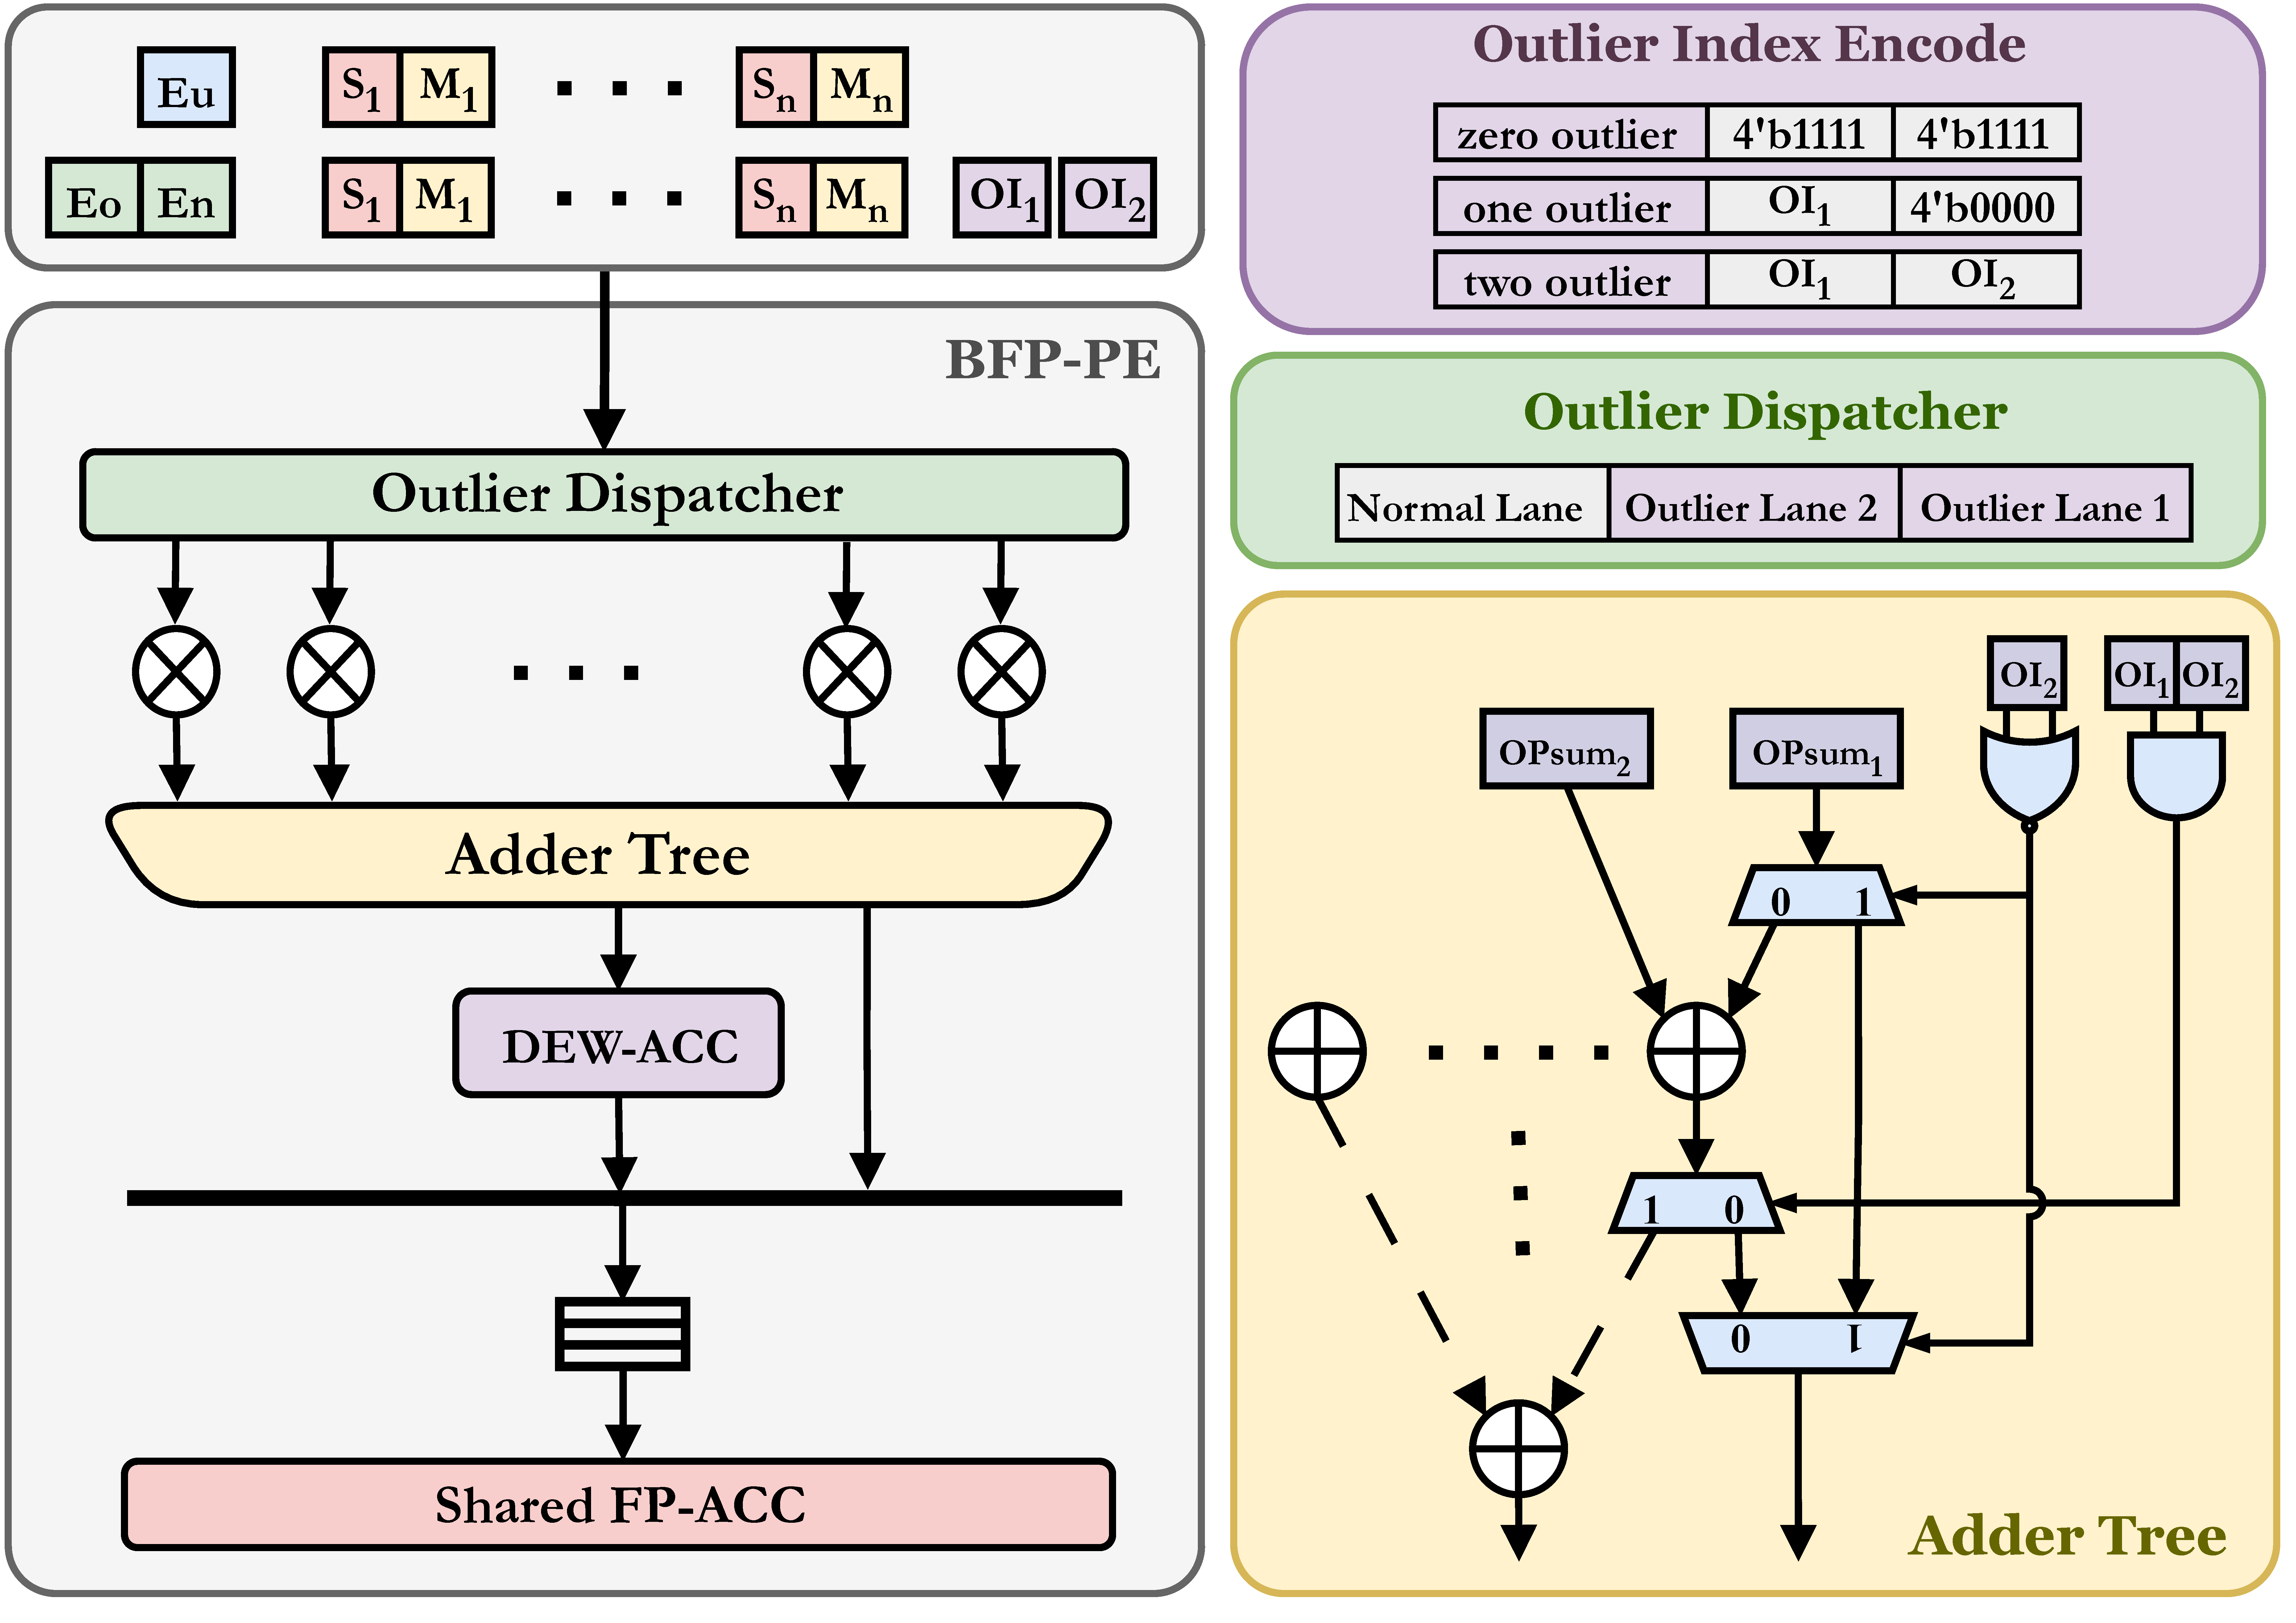
\includegraphics[width=\linewidth]{figures/fig_architecture.pdf}
    \caption{Proposed Top-2 activation routing with asymmetric DEWA and shared FP-Acc.}
    \label{fig:architecture}
\end{figure}
